\documentclass[10pt]{article}
\usepackage{float}
\RequirePackage{eso-pic}
\usepackage{caption}
\captionsetup[table]{labelformat=empty}



\usepackage{geometry}
\geometry{
a4paper,
left=11mm,
right=14mm,
top=37mm,
bottom=14mm,
}



\usepackage{colortbl}
\usepackage{fontspec}
\setmainfont[Ligatures=TeX]{Calibri}



\newcommand\BackgroundPic{%
\put(0,0){%
\parbox[b][\paperheight]{\paperwidth}{%
\vfill
\centering
\includegraphics{MBIE_generic_background.pdf}%
\vfill
}}}



\begin{document}
\thispagestyle{empty}
\AddToShipoutPicture{\BackgroundPic}
\section*{Key Export Statistics\footnotemark - Honey\footnotemark }
\today\\
\begin{table}[ht]
\centering
{\scriptsize
\begin{tabular}[t]{p{1.8cm}>{\hfill}p{1.4cm}>{\hfill}p{1.4cm}>{\hfill}p{1.6cm}>{\hfill}p{1.9cm}>{\hfill}p{2cm}>{\hfill}p{1.9cm}>{\hfill}p{1.5cm}}
 \textbf{Country} & \textbf{Yearly Qty} & \textbf{Yearly Value} & \textbf{Yearly Price} & \textbf{3Year CAGR(Qty)} & \textbf{3Year CAGR(Value)} & \textbf{3Year CAGR(Price)} & \textbf{Price Elasticity} \\
\hline
Australia & 1,452 & 46.9 & \$32.3 & 36\% & 50.8\% & 10.8\% & 3.3 \\  
United Kingdom & 2,040 & 46.8 & \$22.9 & 2.5\% & 19.6\% & 16.6\% & 0.2 \\  
China & 1,476 & 43.9 & \$29.7 & 41.6\% & 67.2\% & 18.1\% & 2.3 \\  
Hong Kong & 1,211 & 35.2 & \$29.0 & 0.7\% & 27.2\% & 26.4\% & 0.0 \\  
USA & 730 & 25.1 & \$34.4 & 25.4\% & 43.3\% & 14.2\% & 1.8 \\  
Japan & 595 & 22.7 & \$38.1 & -2.5\% & 25.3\% & 28.5\% & -0.1 \\  
Other & 1,959 & 61.4 & \$31.3 & -8.2\% & 14.6\% & 24.9\% & -0.3 \\  
Total & 9,463 & 281.9 & \$29.8 & 7\% & 30\% & 21.5\% & 0.3 \\  
\hline
\end{tabular}
}
\caption{\scriptsize Top 6 Honey Markets for year ending November - 2015: Quantity('000 kg) Value(NZ\$Mill), Price and their last 3-Year Growth Rates}
\end{table}


\vspace{-0.7cm}



   \begin{figure}[H]
   \centering
    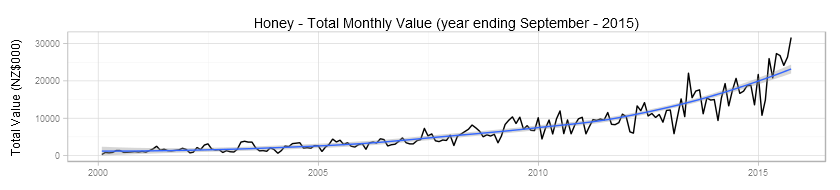
\includegraphics[scale=0.5]{../graphs/monthly_value/honey_monthly_value.png} \
    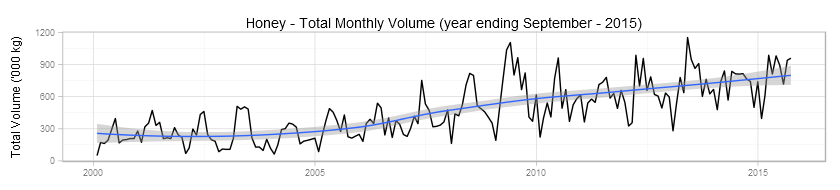
\includegraphics[scale=0.5]{../graphs/monthly_volume/honey_monthly_volume.png} \
    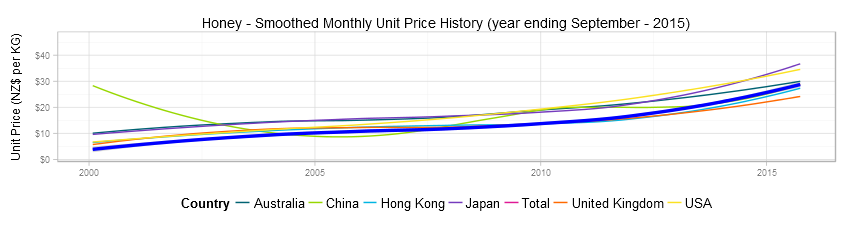
\includegraphics[scale=0.5]{../graphs/smoothed_price/honey_smoothed_price.png} \
    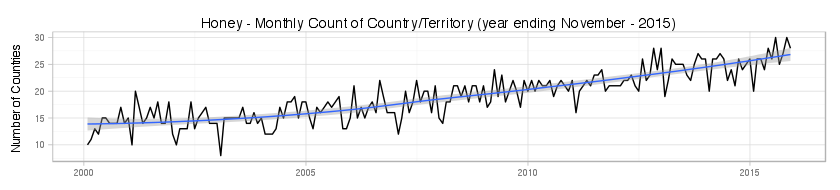
\includegraphics[scale=0.5]{../graphs/monthly_number_countries/honey_monthly_count.png} \
    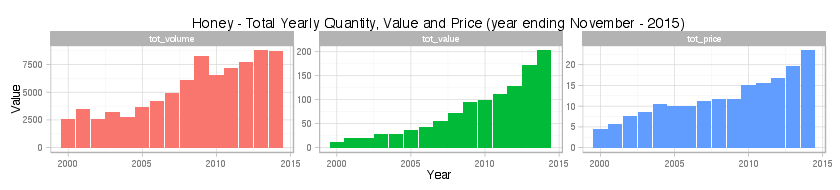
\includegraphics[scale=0.5]{../graphs/yearly_summary/honey_yearly_summary.png} \
   \end{figure}



\footnotetext[1]{Source: Statistics New Zealand - Overseas Merchandise Trade}
\footnotetext[2]{Harmonised System Codes for Honey starting with: 040900.}
\end{document}
